 \begin{frame}{Product Development}{}
    Contributors:
    \begin{itemize}
            \item{Stress}
            \item{Fatigue}
            \item{Motivation}
            \item{Time Pressure}
    \end{itemize}
    Dynamic by generating new schedule quickly
    %We found that stress, fatigue, motivation, time pressure are the biggest contributors to incidents, to help this we can optimize their workday, by generating a schedule, an optimization problem. We simulate dynamic scheduling by generating a new schedule, when changes or incidents occur.
\end{frame}

\section{Technical Delimitation}{
\subsection{Job Shop Problem}{
    %This is a optimization problem, described as job shop problem. Given n jobs J1, J2, ..., Jn of varying sizes, which need to be scheduled on m machines, while trying to minimize the duration of the schedule. with the addition of the being able to assign multiple workers to one task. This is an NP-hard problem, which meant we sought to make the problem as simple as possible, cutting out some variables in order to ensure we can solve it in polynomial time. We tried to find an algorithm for optimizing the process of planning the schedules, by minimezing idle-time og delay-time, this turned out to be quite complex. Changing something early in the schedule, may cause dramatic changes later in the schedule, due to varying durations and dependencies of tasks.

    \begin{frame}{Job Shop Problem}{}
        \begin{itemize}
            \item{Jobs J1, J2, ..., Jn of varying sizes}
            \item{Need to be distrubuted on m machines}
            \item{While minimizing duration of the total schedule}
        \end{itemize}
    \begin{figure} 
            \centering
            \fbox{
            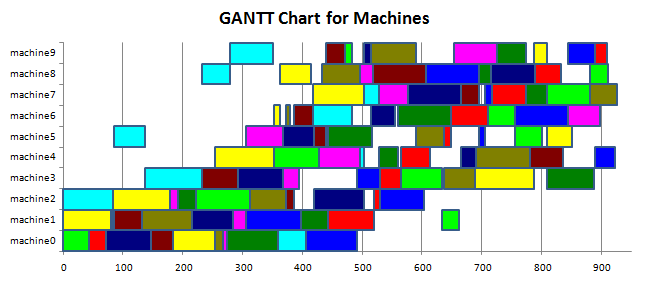
\includegraphics[width=260px]{Grafik/jobshop2}
            }
                \caption{Gantt chart for machines}
            \label{Excel}
        \end{figure}
    \end{frame}
}

\subsection{Algorithms}{
    \begin{frame}{Algorithms}{}
    What we could have used to solve this problem:
    \begin{itemize}
        \item{A genetic algorithm}
        \item{Brute Force Search}
        \item{Most Critical Path algorithm}
    \end{itemize}
    \end{frame}

    \subsubsection{Genetic Algorithm} % (fold)
    \label{sub:genetic_algorithm}
        %We could have used a genetic algorithm for a schedule, which have could have been implemented by the algorithm starting out with two randomly generated drafts of schedules, and then proceeding by performing a crossover of the parent schedules and mutating it into a new possibly better fitted schedule. This would be considered by a obversing element, probably as a function in the algorithm.

        %This being part of evolutionary algorithms, in the artificial intelligence field, we concluded that we didnt have the sufficient knowledge to implement this.
        \begin{frame}{Genetic Algorithm}{}
        \begin{figure}
            \centering
            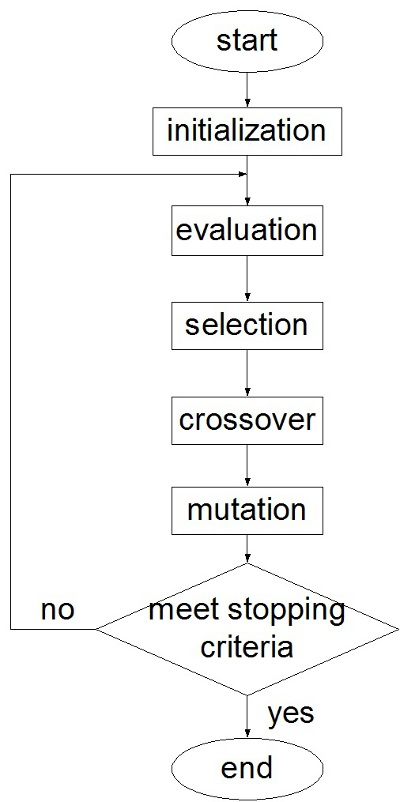
\includegraphics[width=80px]{Grafik/GeneticFlow}
                \caption{A flowchart of a general genetic algorithm}
            \label{GeneticFlow}
        \end{figure}
        \end{frame}

    % subsection genetic_algorithm (end)
    \subsubsection{Brute Force Search} % (fold)
    \label{sub:bruteforce}

    \begin{frame}{Brute Force Search}{}
    \begin{itemize}
        \item{Try every combination of tasks in a huge search space}
        \item{Number one weakness: complexity $O(n!)$}
    \end{itemize}
    \end{frame}

    %We could have used bruteforce, by simply trying all combinations of tasks and picking the most optimal one. But when adding variables and increasing the size of the problem, we figured that the amount of iterations required to find the optimal solution, would be to many and thereby requiring to much time, for it to work in context.

    % subsection bruteforce (end){
    \subsubsection{Most Critical Path} % (fold)
    \label{sub:most_critical_path}

        %Another also possible way to solve the problem is by using the Most Critical Path algorithm, describing dependencies through a directed graph then traversing it by backtracing, finding weights of all nodes in the graph it is then possible to make a priority list for the order of the task how should be executed. Each time a worker is done, the highest priority task is assigned if its dependencies are done. Because of already having a course in discrete mathematics, it seemed pretty straight forward to use a algorithm based in graph theory. Therefore we ended up with the Most Critical Path algorithm with backtracing for solving this problem, due to already known knowledge for making such an implementation and bruteforce not having a sufficient scaling.

        \begin{frame}{Most Critical Path}{}
        \begin{figure}
            \centering
            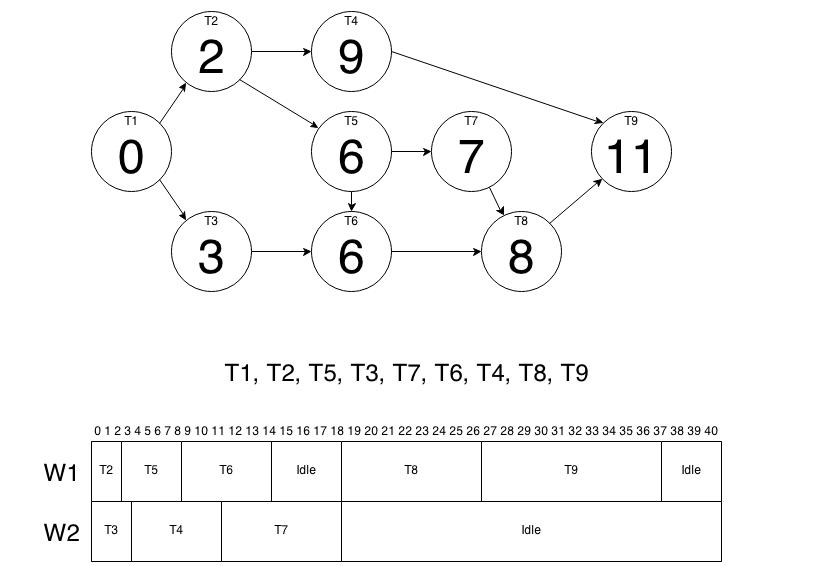
\includegraphics[width=200px]{Grafik/GraphA2}
                \caption{Graph and workers}
            \label{MCP}
        \end{figure}
        \end{frame}

    % subsection most_critical_path (end)
}
}